\documentclass[english]{article}
\usepackage[T1]{fontenc}
\usepackage[utf8]{inputenc}
\usepackage{listings}
\usepackage{graphicx}
\usepackage{etex}
\reserveinserts{100}
\usepackage{morefloats}
\usepackage{dcolumn}
\usepackage{tabularx}
\usepackage{multirow}
\usepackage{array}
\usepackage{chngpage}
\usepackage{booktabs}
\usepackage[spanish]{babel}
\usepackage{verbatim}
\usepackage{moreverb}

\decimalpoint

\let\verbatiminput=\verbatimtabinput
\def\verbatimtabsize{4\relax}

\renewcommand{\tablename}{Tabla}

\newcolumntype{K}{>{\centering\arraybackslash$}X<{$}}


\begin{document}

\makeatletter
\title{Multi-Objective Compact Differential Evolution}
\author{Moisés Osorio}
\date{\today}
\makeatother
\maketitle

\section*{Implementación actual}
La implementación actual está basada en PAES. Ésta funciona así:

\verbatiminput{mocde-main.code}

Donde $F$ es el factor de variación diferencial, $CR$ la razón de cruza, $n$ el número de parámetros de entrada y $np$ el tamaño de la población.

Para determinar si un individuo se agrega al archivo, se realiza lo siguiente:

\verbatiminput{mocde-grid.code}

Este ultimo algoritmo trata de indicar cuándo debe sustituirse el individuo actual por su hijo.

Un factor que se ha mostrado importante, y parece necesitar de calibración, es el tamaño de la desviación estándar inicial utilizada para tomar muestras de la población.

\section*{Resultados}

Varias funciones de prueba se han utilizado para comparar los resultados obtenidos por la implementación actual de mocDE. Las siguientes figuras muestran el desempeño alcanzado por mocDE, MOEA/D, PAES y NSGA-II en comparación con el frente de Pareto real. Así mismo, las tablas muestran la media y la desviación estándar de los resultados de algunas métricas calculadas sobre 20 ejecuciones de dichos algoritmos. Las figuras muestran la mejor y peor ejecuciones de mocDE, de acuerdo a la distancia generacional, junto al respectivo frente de Pareto de cada función de prueba. En la tabla \ref{tab:results-summary} se puede visualizar el resumen de todos los resultados obtenidos.

Los parámetros utilizados para las funciones de prueba son los detallados en la tabla \ref{tab:params}. Donde $n_{var}$ es el número de variables del problema.

\begin{table}
	\centering
        \begin{tabularx}{1\textwidth}{| c || c | K |}
        \hline
            Algorithm & Parameter & Value \\ \hline \hline
            \multirow{4}{*}{\textbf{mocDE}}
                & Evaluations & 300000 \\
                & Population size & 100 \\
                & Differential variation & 0.9 \\
                & Crossover probability & 0.3 \\
                \hline
            \multirow{8}{*}{\textbf{MOEA/D}}
                & Evaluations & 300000 \\
                & Population size & 100 (2-D), 600 (3-D) \\
                & Niche size & 100 (2-D), 150 (3-D) \\
                & Update limit & 10 (2-D), 15 (3-D) \\
                & Differential variation & 1.0 \\
                & Crossover probability & 0.5 \\
                & Mutation rate & 1.0 / n_{var} \\
                & Mating selection probability & 0.9 \\
                \hline
            \multirow{6}{*}{\textbf{PAES}}
                & Evaluations & 300000 \\
                & Archive size & 100 \\
                & Mutation rate & 0.01 \\
                & Grid depth & 4 \\
                & Gene length & 30*n_{var} \\
                & Number of alleles & 2 \\
                \hline
            \multirow{4}{*}{\textbf{NSGA-II}}
                & Evaluations & 300000 \\
                & Population size & 100 \\
                & Mutation rate & 0.01 \\
                & Crossover probability & 0.9 \\
                \hline
        \end{tabularx}
    \caption{\label{tab:params} Algorithm parameters.}
\end{table}

%RESULTS%

El progreso en los resultados puede ser condensado como se muestra en la figura \ref{fig:progress}.

\begin{figure}
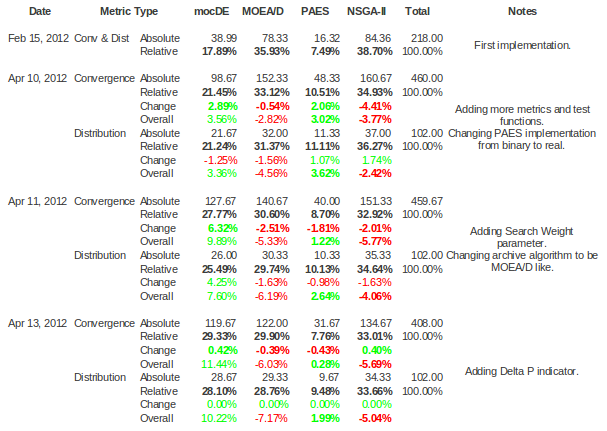
\includegraphics[scale=0.6]{images/progress}
\caption{\label{fig:progress} Result progress.}
\end{figure}


\section*{Trabajo actual}

Actualmente se tienen los siguientes objetivos:
\begin{itemize}
\item Investigar funciones de densidad para saber cuándo reemplazar una solución por otra.
\item Revisitar la escalarización de Chebyshev ya que se encontró un error de implementación en ella.
\item Investigar operadores y técnicas utilizadas en micro algoritmos genéticos.
\end{itemize}

\section*{Cronograma de Actividades}

Las actividades a realizar durante el trabajo de tesis son:
\begin{enumerate}
\item Revisión del estado del arte y literatura relacionada. Obtener un panorama amplio del trabajo pasado y actual sobre la optimización multiobjetivo, a fin de compararse y mejorar, de algún modo, dichos trabajos.
\item Diseño general del algoritmo principal. Definir de manera general, el enfoque de solución a utilizar.
\item Implementación básica capaz de resolver problemas sencillos. Implementar una versión del algoritmo que sea competitiva en problemas generalmente reconocidos como fáciles.
\item Redacción del protocolo de tesis. Definir el problema, el alcance del trabajo de investigación y el plan general de trabajo.
\item Implementación de scripts de pruebas y estadísticos. Implementar scripts que permitan obtener valores estadísticos sobre el desempeño del algoritmo, a fin de ser comparado con el estado del arte.
\item Mejora de la convergencia de la implementación básica. Mejorar la convergencia de los resultados obtenidos por el algoritmo, a fin de que sea competitivo en problemas más difíciles que aquéllos resueltos por la versión básica.
\item Mejora de la distribución de la implementación mejorada. Aumentar la distribución de los resultados obtenidos por el algoritmo ya que, como la convergencia, éste es otro indicador de la calidad de los mismos.
\item Escritura de tesis. Redactar aquellos capítulos que no necesiten de los resultados finales del algoritmo.
\item Refinamiento general de la implementación del algoritmo. Refinar los últimos detalles del algoritmo para alcanzar su máxima eficacia y eficiencia.
\item Finalización de escritura de tesis. Redactar aquellos capítulos finales dependientes de los resultados del algoritmo.
\item Publicación de resultados. Escribir un artículo en un congreso internacional para dar a conocer los resultados de esta investigación.
\end{enumerate}

La figura \ref{fig:calendar} muestra el cronograma de las actividades anteriormente detalladas. La región verde es aquella que ha sido completada, la roja es la que se está trabajando actualmente y la gris aquella por realizar.

\begin{figure}
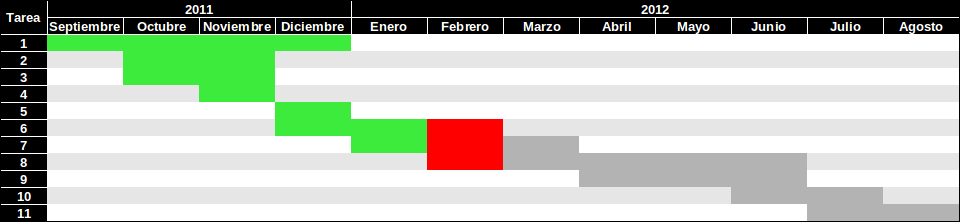
\includegraphics[scale=0.5]{images/cronograma}
\caption{\label{fig:calendar}Cronograma de actividades.}
\end{figure}

\end{document}
